\documentclass[preprint,10pt]{elsarticle}
\usepackage{etoolbox}
\makeatletter
\patchcmd{\ps@pprintTitle}{\footnotesize\itshape
       Preprint submitted to \ifx\@journal\@empty Elsevier
       \else\@journal\fi\hfill\today}{06.2018}{}{}
\makeatother

\usepackage[margin=2.5cm]{geometry}

\newcommand{\fscale}[1]{#1\linewidth}
\newcommand{\figref}[1]{Fig.~\ref{#1}}

%-----------------------------------------------------------------------------
%  Colors
%-----------------------------------------------------------------------------
\usepackage{pagecolor}
\definecolor{linen}{RGB}{240,240,230}
\definecolor{fwhite}{RGB}{255,250,240}
\definecolor{oldlace}{RGB}{253,245,230}
\definecolor{awhite}{RGB}{250,235,215}
\definecolor{pwhip}{RGB}{255,239,213}
\definecolor{peach}{RGB}{255,218,185}
\definecolor{ivory}{RGB}{255,255,240}
\definecolor{seashell}{RGB}{	255,245,238}

\usepackage{sectsty}
\sectionfont{\Large \textsf}
\subsectionfont{\large \textsf}

\usepackage{amsmath}
\newcommand{\mr}[1]{\mathrm{#1}}  % Roman font for the math mode
\newcommand{\mi}[1]{\mathit{#1}}  % Italic font for the math mode
\newcommand{\mc}[1]{\mathcal{#1}} % Caligrafic (script) font for the math mode
\newcommand{\ms}[1]{\mathsf{#1}}  % Sans font for the math mode (vectors and matrices)
\newcommand{\mb}[1]{\mathbf{#1}}  % Bold font for the math mode (vectors and matrices)

\usepackage{mathtools}
\DeclarePairedDelimiter\ceil{\lceil}{\rceil}
\DeclarePairedDelimiter\floor{\lfloor}{\rfloor}

\usepackage{amsthm}
\theoremstyle{definition}
\newtheorem{definition}{Definition}[section]
\newtheorem{remark}{Rule}[section]

\newtheorem{property}{Property}

\newtheorem{theorem}{Theorem}

\usepackage{cleveref}
\crefformat{section}{\textbf{\S#2#1#3}} % see manual of cleveref, section 8.2.1
\crefformat{subsection}{\textbf{\S#2#1#3}}
\crefformat{subsubsection}{\textbf{\S#2#1#3}}

\renewcommand{\cref}[1]{\textbf{\S\ref{#1}}}

\usepackage{graphicx}
\usepackage{subfigure}
\graphicspath{{./fig/}}
%% The amssymb package provides various useful mathematical symbols
\usepackage{amssymb}

\usepackage[titletoc]{appendix}
\usepackage[T1]{fontenc}

\usepackage{xcolor, soul}
\sethlcolor{oldlace}

\usepackage{lineno}
\usepackage{url}
\bibliographystyle{unsrt}

\patchcmd{\abstract}{Abstract}{Summary}{}{}

\begin{document}

\begin{frontmatter}

%% Title, authors and addresses

\title{\textsf{Latitude: A Blockchain for the Transportation Industry\tnoteref{title1}}}
\tnotetext[title1]{Full whitepaper Version 2.0}

\author{Latitude Labs\corref{auth1}}
\cortext[auth1]{Latitude Labs at https://latitude0x.com}
\address{Silicon Valley, California}

\begin{abstract}

Blockchains are rapidly becoming the new vehicles for decentralized applications for the data sharing economy. By their
    design, they are able to create privacy aware, secure, trusted, verifiable and user incentivized ways of sharing
    data. This ability has created a new wave of applications in various industries which are disrupting the status quo
    of the incumbents. Also, the Transportation industry is seeing a shift in terms of the amount of data that has
    become available due to mobile phones, dedicated sensors and crowd-sourced availability of data. The industry has a
    large number of applications, users and regulations which can benefit from data sharing if it can be done correctly.

 We present the Latitude blockchain which is designed to be the best blockchain for transportation applications.
    Latitude is designed using principles derived from the core decentralized blockchain technologies available today
    combined with fundamental considerations for the unique aspects of Transportation data and applications. Latitude
    includes the world's first smart contract system specifically tailored for geo-spatial, mapping, location and sensor
    data and related applications. The system is powered by a geo-spatial decentralized datastore which can scale to
    planet level storage capabilities incentivized by a token economics built over the LAT (Latitude Token).

    The Latitude network is also provisioned with a library of algorithms, both open source and closed form, which allow
    Government, insurance companies and regulators to compute, certify and create cryptographic proofs which can help enforce policies
    or verify contracts.  Latitude has a decentralized Governance model using a Council system which is resistant to
    collusion and Byzantine behavior and is incentivized to maintain honest and proper operation of the network.

    Latitude can support four classes of applications. First, Ridesharing applications consist of the sharing economy
    applications for multi-modal ridesharing and transport. Using Latitude, it becomes possible to create better
    incentives for ride providers and users including incentives for data sharing and route optimizations. This also
    allows regulatory bodies to participate in the execution of these applications using smart contracts. Second,
    Telematics applications such as Usage-based Insurance (UBIs) and fleet management can benefit from real-time or
    historical data and corresponding intelligent algorithms, thus providing shared mutual benefits. The third class of
    application include mapping and location.  Using tangible user incentives while providing strong trust, privacy and
    security for user data, it is possible to create new or better data sharing applications (similar to Waze among
    others) on the Latitude platform. Finally, all the geo-spatial, location, mapping and real-time city level data can be used by the City and State
    governments for smart city applications to provide a better quality of life for their citizens.
\newline \newline \newline \end{abstract}

\begin{keyword}
	\textsf{location \sep cryptography\sep decentralization \sep blockchain \sep ethereum \sep database \sep sql
    \sep access control \sep p2p \sep tokens \sep incentives \sep mechanism design \sep byzantine
    faults \sep data sharing \sep latitude \sep longitude \sep driverscore \sep mapping \sep transportation \sep
    insurance}
\end{keyword}

\end{frontmatter}

\newpage
\tableofcontents
\newpage

%-----------------------------------------------------------------------------
%  INTRODUCTION
%-----------------------------------------------------------------------------
\section{Introduction}\label{sec:intro}

- There is a fundamental shift happening in the transportation industry. Automation, data, AI based analytics.
- Centralized solution examples:
    - Telematics data exchanges.
    - Mapping and location data: privacy security issues. Lack of user control.
    - Centralization creates DATA SILOS. Explain and expand.
- What powers this is data, being able to share data, analytics, computation using AI, in a trustworthy privacy-aware
manner.

- The industry needs a solution that can allow new ways of sharing the data while providing strong unbreakable gurantees
of security privacy etc.


- Overview of our solution:
  - Blockchains can provide these gurantees and much more. 
  - Examples of other industries where blockchain is posed to disrupt traditional data sharing:
    - IOT example.
    - Supply chain management.
    - Renting.
  - Section level overview.



We are in the midst of building a new Internet. Blockchain networks like Ethereum have popularized the idea of unstoppable, owner less applications that are run on an open network of untrusted but incentivized nodes without the oversight of a central authority. An increasing number of these decentralized applications (\DJ apps) are being created everyday with evolving data storage needs. The first generation of these dapps stored their data entirely on a blockchain itself while the current ones are storing it on decentralized file storage systems like IPFS with just hashes of the data stored on the blockchain. Although this method works for dapps with simple storage needs like the need for storing data as a blob, it is very limiting for dapps with more complex requirements such as the need to store data at a more fine grained level and efficiently querying it. A popular option is then to use a cloud hosted database (ex: Google’s Cloud SQL) but that turns a dapp into a non-dapp by introducing centrality into the system. \newline\newline

Rest of the paper is structured as follows: in section 2, we discuss some related work. Section 3 presents the overall design of the system, section 4 presents the network subsystem, section 5 presents the database subsystem and section 6 presents our approach to dealing with problems that arise in a network made up of untrusted nodes and discusses an incentive mechanism to make them behave as per system's needs. In section 7, we propose a message exchange protocol in the same vein as http but for relational data sharing. Section 8 concludes the paper.


The introduction of Bitcoin \cite{nakamoto2009bitcoin} has triggered a new wave of decentralization in computing. 
Bitcoin illustrated a novel set of benefits: decentralized control, where ``no one'' owns or controls the network; immutability,
where written data is tamper-resistant (``forever''); and the ability to create \& transfer assets on the network, without reliance on a central entity.

The initial excitement surrounding Bitcoin stemmed from its use as a token of value, for example as an alternative to government-issued currencies.
As people learned more about the underlying blockchain technology, they extended the scope of the technology itself (e.g. smart contracts), as well as applications (e.g. intellectual property).

With this increase in scope, single monolithic ``blockchain'' technologies are being re-framed and refactored into building blocks at four levels of the stack:
\begin{enumerate}
 \item Applications
 \item Decentralized computing platforms (``blockchain platforms'')
 \item Decentralized processing (``smart contracts'') and decentralized storage (file systems, databases), and decentralized communication
 \item Cryptographic primitives, consensus protocols, and other algorithms
\end{enumerate}




\section{Background on Blockchain}\label{sec:blockchain}

Blockchain has the potential to become the new decentralized application platform over the Internet. Blockchain is a public register in which transactions between two users belonging to the same network are stored in a secure, verifiable
and permanent way. The data relating to the exchanges are saved inside cryptographic blocks, connected in a hierarchical
manner to each other. This creates an endless chain of data blocks -- hence the name blockchain -- that allows you to
trace and verify all the transactions you have ever made.

The introduction of Bitcoin \cite{nakamoto2009bitcoin} triggered a new wave of decentralization in computing.
Bitcoin illustrated a novel set of benefits: decentralized control, where ``no one'' owns or controls the network;
immutability, where written data is tamper-resistant (``forever''); and the ability to create \& transfer assets on the
network, without reliance on a central entity.

The initial excitement surrounding Bitcoin stemmed from its use as a token of value, for example as an alternative to
government-issued currencies.  As people learned more about the underlying blockchain technology, they extended the
scope of the technology itself (e.g. smart contracts), as well as applications (e.g. intellectual property).

Bitcoin was the first such blockchain to introduce concept of full decentralization, but Ethereum has made this a
general platform for executing arbitrary applications called dapps using smart contracts and a wide range of other
tools. Since Ethereum, there has been an explosion in blockchain technology to allow a wide range of distributed
decentralized applications to run over a network of untrusted arbitrary nodes over the planet, which almost mimic the
structure and spread of the Internet.

%Blockchain is a
%public register in which transactions between two users belonging to the same network are stored in a secure, verifiable
%and permanent way. The data relating to the exchanges are saved inside cryptographic blocks, connected in a hierarchical
%manner to each other. This creates an endless chain of data blocks -- hence the name blockchain -- that allows you to
%trace and verify all the transactions you have ever made.

 The primary function of a blockchain is, therefore, to certify transactions between people. In the case of Bitcoin, the
 blockchain serves to verify the exchange of cryptocurrency between two users, but it is only one of the many possible
 uses of this technological structure. In other sectors, the blockchain can certify the exchange of shares and stocks,
 operate as if it were a notary and "validate" a contract or make the votes cast in online voting secure and impossible
 to alter.
- Introduce the concept of decentralization, bitcoin, ethereum and blockchains in general.

Decentralization is one of the core concepts or features of a blockchain. It can mean different things in different
contexts but for our purposes it allows for (1) decentralization of control or power, that, (2) decentralization of
software.

{\em Why is decentralization useful ?}
\begin{itemize}

    \item Fault tolerance - decentralized systems are less likely to fail accidentally because they rely on many separate
components that are not likely.
    \item Attack resistance - decentralized systems are more expensive to attack and destroy or manipulate because they lack
sensitive central points that can be attacked at much lower cost than the economic size of the surrounding system. This
can be important for transportation data as it does not remain under a single point of failure.
    \item Collusion resistance:it is much harder for participants in decentralized systems to collude to act in ways that
benefit them at the expense of other participants, whereas the leaderships of corporations and governments collude in
ways that benefit themselves but harm less well-coordinated citizens, customers, employees and the general public all
the time.
\end{itemize}

One of the key concepts of blockchains becoming an application platform is smart contracts. A standard contract, as a
legal document, binds two or more parties into an obligation to achieve certain deliverables or outcomes. A smart
contract is a piece of code that similarly binds multiple parties into outcomes that are verifiable, computable or
provable using code and strong cryptographic constructs. Ethereum was the first such platform to introduce the concept
of smart contracts which has since been adopted by most other blockchains that wish to host decentralized applications
(dapps).

Because smart contracts can be executed by arbitrary nodes on the blockchain, its possible for anyone to "verify" the
smart contract. This createst the concept of trust using consensus. Consensus is defined as the agreement among a
certain number (or fraction) of nodes on a particular result or outcome. With consensus, it becomes much harder for a
Byzantine or adversarial node \cite{lamport_byz} to manipulate the smart contract in ways that was not intended or
provisioned for. One of our goals, as discussed later in Section \ref{sec:design} is to build a smart contract framework
that is tailored for Transportation applications, so that the contracts are readily available, trustable and
enforceable. 

Smart contracts can allow new ways of data sharing that were not possible before. By creating strong programmatic
constructs combined with consensus protocols and cryptographic primitives it is possible to share data in a way that
privacy, security and restrictions on use can be enforced. There has been a lot of recent progress on how to use Smart
Contracts for data sharing \cite{liu_2018}. Thus, the technology today is ready for creating disruptive new ways of
sharing transportation data to create new applications such as smart cities, driver behavior, insurance, mapping etc.
This technology can be disruptive to incumbents who might be late for adoption.

- Concepts of smart contract, trust, consensus.

- How data sharing can work in a blockchain manner. 
- Overview of cryptographic proofs. How they work.
- Discussion of Byzantine behavior.

-Blockchain based Platform is decentralized.
    - No single point of control or failure.
    - Users own their data and reputation.
    - Every functionality is openly verifiable.

- System is open-source
 - Every entity knows how data, algorithms and logic is implemented.
 - Policies can be verified using Trusted Computing.

- Anyone can participate including Governments, Individuals, Enterprises.
- Governance happens using a council of participants.
- Privacy and Security policies can be enforced through strong cryptographic primitives.


- Smart contracts allow for precise enforcement of incentives, data sharing and privacy protection.
- Industry or Government Standards are enforceable and verifiable.
- Raw and derived data can outlive the companies or geographies.
- Eg: DriverScore can carry over to a different country or geography.
- Mapping data can be utilized outside of the GIS provider.




\section{The Latitude Blockchain}\label{sec:design}

In this section, we present a high-level design of the Latitude blockchain. The full-version of this whitepaper shall
contain a very detailed design of each component. We start with an overview of the key design principles that will guide
the rest of the design for the Latitude Blockchain. Its important to note here that for implementation purposes, it
might be possible to use an existing core blockchain for the underlying functionalities and build Latitude as a layer on
top. We shall make these determinations in the full-version of the whitepaper.

\subsection{Design overview}

The purpose of the Latitude blockchain is to become the best platform in the world for decentralized applications for
the Transportation Industry. Specifically, this boils down to constructs in the blockchain that can handle spatial,
mapping, traffic, driving data including data relating to other modalities of transport (bike sharing, walking, even air
routes later on). Figure XXX presents the architecture of the Latitude blockchain in terms of the core technological
innovations that will be built into it.

\begin{figure}[t]
    \centering
    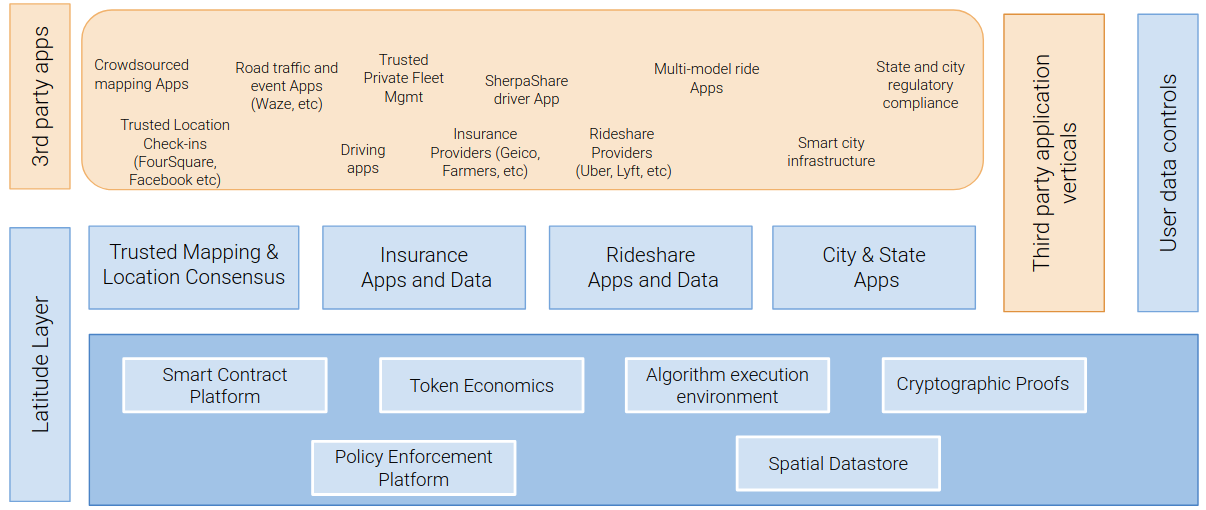
\includegraphics[width=0.90\textwidth]{latarch.png}
  \caption{Architecture of the Latitude Blockchain and associated platform ecosystem.}
    \label{fig:lat-arch}
\end{figure}

One of the central aspects of the Latitude blockchain is a geo-spatial datastore that fundamentally understands various
datatypes that are specific to transportation data. This datastore can use existing GIS databases that allow
de-centralized storage and access. The types of data include (i) georaphic data such as location (latitude, longitude),
(ii) mapping data such as roads, terrain, addresses, etc, (iii) sensor data such as driving data, driver score, miles
driven, route information, etc, (iv) multi-modal transport data such as biking, walking and other means of transport.
Each of these data types have very special characteristics which the underlying datastore can be optimized for and allow
for programming using what we call the {\em Latitude Smart Contract} framework. 

The datastore would include spatial, quad-tree or an R-tree based indexes for efficient querying and other operations that
most Geographic Information Systems (GIS) would support in a centralized manner today. It would also include functions
to compute heatmaps, driving maps and statistics such as Traffic predictions including real-time analytics. Depending on
how Latitude evolves, the datastore can include additional functionalities to support the data sharing among autonomous
vehicles since they use most of the similar datatypes mentioned above. The datastore would support circular, rectangular
and other range queries, K-nearest neighbor searches, route optimization algorithms, etc. Figure
\ref{fig:geo_spatial_query} shows some of the queries that such a datastore can support.

\begin{figure}[t]
    \centering
    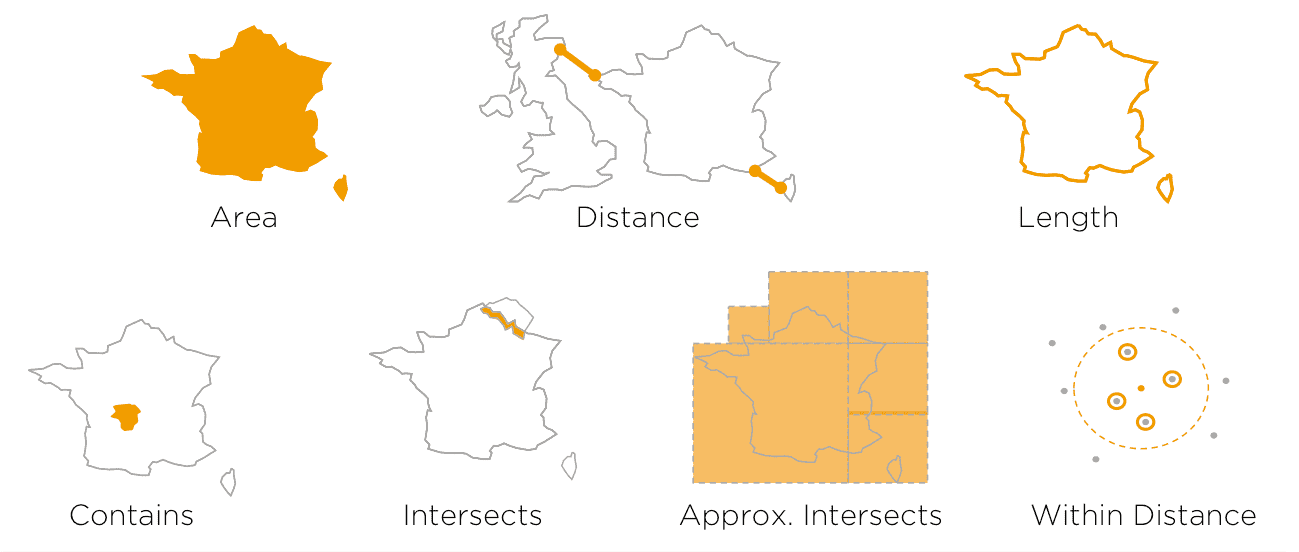
\includegraphics[width=0.90\textwidth]{geospatial_query.png}
  \caption{Examples of Geo-spatial queries that a spatial datastructure can support on the Latitude blockchain.}
    \label{fig:geo_spatial_query}
\end{figure}


Datastore
 - Optimized for Geographic, Geo-spatial data.
 - Location, Mapping data and computation.
 - Ability to Store, index, query and build smart contracts optimized for such data.
 - Support for various spatial indexes.
 - Location heatmaps.
 - Indexing road and driving data.
 - Primitives for storing driving data for autonomous vehicles

\noindent
{\textsf Strong crytographic foundation:}
Standard data encryption techniques allow for security guarantees in Latitude. Anonymity guarantees are provided using
privacy-preserving set operations such as given in \cite{kissner_set}, with suitable modifications to
anonymize spatial data which have user-location considerations \cite{divanis_kanon,xu_loc_anon}.
Cryptographic primitives for:
 - Security and privacy of data.
 - Anonymity guarantees using cryptographic set operations.
 - Enforcement of privacy when sharing data.
 - Sharing of “computation” instead of data when possible.
 - For eg: Sharing of DriverScore using a vetted algorithm.
 - Sharing proximity to a landmark instead of lat/lng.
 - Ability to find bad actors.
 - Detect privacy, anonymity and security violations.

\noindent
{\textsf Latitude Smart contract system:}

Smart contract system for Transportation applications.
 - Ability to convert “policies” such as GDPR into smart contract code.
 - Example, self destruct data after a time period.
 - Sandboxed trusted execution environment:
 - For algorithms:
   - DriverScore, Location heatmaps, Statistics.
   - Enforcing or verifying privacy and other govt policies/regulations.

Cryptographic proofs for applications:
 - Proof of Location. 
 - Proof of ride. 
 - Proof of mapping 
      (road/landmark exists or does not exist).
 - Proof of driver score 
 - Open, trusted, understood driver score computation algorithms.
 - Cryptographic proofs can be shared among entities, safely, securely.

\noindent
\subsection{Cryptoeconomics and Governance:}
Cryto-economics refers to the mechanics of the protocol underlying the blockchain operations which creates incentives
for the various stakeholders. For example, in the Latitude Blockchain it is possible to reward users for sharing their data
for certain purposes. For example, users can be rewarded if they share traffic data or accident information or better
routes. This is similar to the Waze model but creates legitimate rewards for users that have meaningful value outside
the Waze application. For an overview of cryptoeconomics in the blockchain space, please see \cite{sinclair_crypto}.

The core building block of the cryptoeconomics in Latitude is the Latitude Token, or LAT. This will be transacted in
each and every micro-transaction that takes place on the blockchain to create the right incentives, enforce smart
contracts and penalize Byzantine behavior. One of the fundamental design principles behind the protocol for the LAT
token is to create incentives assuming nodes are greedy and are interested in maximizing their gain. We will also build
safeguards against reasonable amount of collusion among nodes to subvert the system. The design is crafted such that the
best way for a node to maximize its revenue would be to participate with full honesty.

Latitude shall employ a Proof of Stake model (delegated or non-delegted) for particpation and core node-level mining. This mechanism has recently
gained popularity among a notable number of blockchains \cite{dpos_steemit}. This also allows for deposit slashing as a
technique to tackle Byzantine behavior. Latitude will employ techniques such as Minimal Slashing \cite{buterin_slashing}
for Byzantine fault tolerance and safety under distributed asynchronous operation.


Governance refers to a decentralized manner in which decisions are made using a consensus mechanism on the blockchain.
Decisions include basic constructs whether a node can join or leave the network. Or it can include key decisions on
whether an upgrade should be mandated on every node, a given participant such as a data provider should be penalized. It
could also include issues where humans get involved, such as when a user complains of a loss of privacy or a breach in
contract.

Recently blockchains have been moving towards governance using a small set of participants, such as trusted miners in
the case of Stellar and Ripple \cite{stellar_gateway}. The EOS blockchain uses a similar concept of a core set of block
producers who are elected based on a nomination and voting process \cite{eos_producers}. For discussion around
Governance in Ethereum, refer to \cite{buterin_gov}. Latitude uses a similar concept of a {\em council} of participants.
These are entities (nodes or organizations) that have demonstrated participating using earned trust through honest
operation, accumulating stake, demonstrated good intent and establishing trust. Some members of this council might
include the core Latitude developers which allows them to implement operations such as updates, bug fixes and so on. The
council members shall be elected using the an election protocol on the blockchain. It might be possible to directly
nominate certain council members such as regulatory bodies who have general interest in user rights, privacy and
enforcement. 

 - Crypto-incentives for honest operation.
 - Penalties for malicious intent.
 - Governance based on consensus and roles using a council.
 - Council members elected using voting, stake and established trust.
 - Some council members can have restricted access.
 - Eg: US govt can have voting rights on US data/users, etc.

User incentives:
 - Users have full control over their data and computation.
 - Users can issue or request proofs to carry over to other applications.
 - User’s have incentive to share data, participate in improving the common denominator.
 - Malicious intent, Byzantine behavior.
   - Can be detected using a combination of consensus and incentives.
   - Best interest of users to act honestly by design.


\noindent
{\textsf Performance considerations:}
Performance:
- Transaction speed. Data throughput. Storage capabilities.


\section{Applications}
\label{sec:apps}

In this section, we discuss the four different classes of applications that can be built on the Latitude platform. Each
of these applications is supported by a suite of software modules, smart contract addons and SDKs (mobile and desktop)
that utilize the core functionality offered by Latitud and provision it in unique ways to suit the specific class of
applications. The Latitude platform is extensible in the sense that its not limited to these four classes of
applications. For example, its possible to add additional applications such as for the shipping or the airline industry
as verticals on the platform. Next we discuss each of these applications and how they can be supported on the platform.

\subsection{Rideshare applications}

Ridesharing applications are the pinnacle of the applications in the data sharing economy. They empower the user to
choose from a multi-modal ways of finding or providing rides. Latitude can provide the decentralized infrastructure to
store, share and build decentralized applications for their corresponding counterparts.

The ridesharing market alone is large enough to power the Latitude blockchain as its primary usecase. The ridesharing
market is around 17 Billion dollars with around 60 Million users. This does not include the multi-modal ride sharing
segment which is growing rapidly. This segment includes bike, scooter and such modes of transport. The ARPU is around 
293 dollars which is high enough to create user incentivized models for data sharing. The data generated by these users
currently sits in silos in the respective ride sharing apps, which can be unlocked and put to good use through such
mechanisms. 

Latitude shall provide a mobile SDK and a blockchain API specifically to suit ridesharing apps for sharing data. This
would allow the creation of decentralized ride sharing apps that can provide users with incentives to share data,
subsidize rides and provide a better deal for ride providers. They can also allow regulators to enforce the use of
roads, lanes, parking and other structures in accordance with city or neighborhood ordinances. Latitude's SDK shall also
provide a multi-modal ride API that such apps can use to request rides on the platform.

As an preferred third-party integration, Latitude shall integrate with SherpaShare's platform for drivers. This would
allow greater sharing of the geo-spatial and driving data collected through SherpaShare's driver app. This will be one
of the early launches for the beta version of the Latitude platform.

%Overview of ridesharing applications. Big industry leaders. Statistics on rides, miles, revenue, ARPU.
%
%Multi-modal ride data:
% - Bike, scooter ride apps.
%Disruptive to Bikesharing:
% - Mobike, OFO, BlueGoGo, Youon, Mingbikes
% - Hellobike, YooBike, CCbike, Zagster, LimeBike
% - Citi Bike, Capital Bikeshare, Divvy, Hubway, Docomo Bike
%Share, Relay Bikes
% - Public transit data
%Use SDK/app to share data. Similar incentive model.
%Monetization:
% - Single multi-modal ride API (SherpaShare or 3rd party).
%
% Ridesharing platform:
%
% Platform:
%Latitude Ridesharing SDK.
%Ridesharing sidechain on the Latitude blockchain.
%Riders:
%Contributing ridesharing data:
%Uber, Lyft, Gett, Juno, Curb, Sitbaq
%Drivers:
% - Use SherpaShare app or 3rd-party app with SDK.
% - Proof of ride:
%Using driver-side app and/or client app.
%Other players:
% - City, Law enforcement, analytics use cases.

\subsection{Telematics applications}

Data is the most important asset for Telematics applications. Thus, sharing of data, computations and algorithms can be
beneficial to companies, users and the ecosystem in general. In fact, by using the Latitude blockchain it becomes
possible for regulators to enforce laws better while maintaining data privacy. This can result in lower crime rates and
incidents.

The important of data sharing here can be seen from the existence of {\em Telematics data exchanges} that are
centralized cloud-based exchanges which act as data brokers among users and insurance companies. As an example, consider
the Verisk Data Exchante (verisk.com) which allows the exchange of driver data to insurance companies. They share data
for all kinds of connected vehicles for underwriting, rating, and claims handling through Usage-based Insurance (UBI)
programs.  The exchange stores and processes telematics data of all types, volumes, and velocity from connected cars,
aftermarket hardware, or mobile solutions. A second example is the Octo Telematics company which also operates an
exchange that is used by over 100 insurance companies, has about 186 billion miles of driving data and gets 11 billion
new data points from 5.4 million connected cars and sensors every day.

The problem with such centralized solutions is that there is a central entity that extracts the fees and has direct
control over the data. Such centralization can result in security and privacy loss and lack of trust from all parties
involved. Latitude is directly poised to disrupt this market by providing a blockchain based platform for exchange of
data, computation, algorithms and resulted information. Using Latitude smart contracts it becomes possible to enforce
proper security, privacy and sharing of data in accordance with agreed upon incentives. This implies cleaner and better
sharing methods which can be a win-win for everyone in the industry including the regulators.

Latitude shall provide a Telematics SDK and blockchain library module to enable such applications. This would include a
suite of pre-existing smart contracts, datastore provisions and other software modules necessary to build decentralized
data exchanges which can eliminate the expensive data brokers. The SDK shall also include APIs for Usage-based Insurance
companies to act as data providers given appropriate involvement, permission and incentives for the users. Users can
also be incentivized to provide data directly to the platform by getting token rewards. Such a model also allows for
open experimentation with driver behavior algorithms such as DriverScore. It also becomes possible for drivers and users
to "carry" their score or reputation from one platform to another, thus preventing lock-in scenarios.

%---Telematics data sharing:
%Data sharing can result in better algorithms, better understanding among drivers.
%Telematics data can save lives:
%Allows government regulations to be enforced. Data privacy can be enforced.
%Driver’s own their driving history (score) and can choose to carry it.
%
%
%---UBI methods can be improved with data sharing and incentives.
%Example:
%Octo telematics
%20 million miles, 186 billion miles of driving data
%100 insurance companies (data is not shared).
%11 billion new data points daily from 5.4 million connected cars and sensors.
%Disruptive opportunity for data sharing.
%
%
%
%---Telematics data exchanges exist today !
%But centralized, unclear policies, enforcement.
% Lack of control.
% Example: Verisk Data Exchange (verisk.com)
% The first-of-its-kind  exchange draws driving data from all kinds of connected vehicles for underwriting, rating, and
% claims handling through UBI programs. 
% The exchange is scalable to normalize, process, and store telematics data of all types, volumes, and velocity from
% connected cars, aftermarket hardware, or mobile solutions.
% Finally, one exchange solves the many-to-many challenge by connecting automakers and telematics service providers
% (TSPs) to multiple insurers
%
%
% ---Insurance Vertical
% Latitude Driver SDK:
% Allows trusted capture of driving data.
% Platform for running DriverScore / Behavior algorithms on phone or in the cloud (or a combination). 
% Eg: Geico:
% Can run 3rd-party algorithms such as Geico’s driver score directly on the phone.
% Includes API for interacting with Geico’s app.
% Users mine currency by:
% Contributing driver data, driver scores.
% Users own the data, have full control.
%
% Insurance providers (Geico, Progressive, Farmers, etc)
% Use platform for computing metrics.
% Contribute data/and or crypto-currency incentivized.
% Always user permissioned.
% Other players:
% City, Law enforcement, analytics use cases.
% Car history use cases (better version of Carfax).


\subsection{Mapping and Location}

Waze example:
 - 70 Mil users, 500k volunteers share data. user spends 480 min/month.

-- Upcoming mapping applications include:
 High-resolution data for self-driving technology.
 Road data, needs consensus and trust.
 Proof of location:
 Location enabled maps. 
 Foursquare checkins. Facebook checkins.
 Location-based access control.
 3 BILLION location requests daily on Android
 250M location-enabled service users.

--Latitude Mapping + Location SDK
Mobile SDK for trusted mapping + location.
SherpaShare app + 3rd party apps.
Users mine by:
Contributing road, traffic, street, mapping data.
Contributing user location
Proof of location concept can replace “Check-Ins”
Facebook has 50 million check-ins per year.
City, law enforcement, analytics use cases.
User has full privacy control.

-- Applications:
Waze like apps:
By Latitude Mapping/Location Sidechain.
Waze, OsmAnd, Maps.Me, HEREWeGo, 2GIS
Yandex.Maps, Locus Maps.
 Navmil, NavIt, MapQuest.
 Crowdsourced maps.
 Authenticated location applications:
 Access control or privileges by virtue of location.

\subsection{Smart city and Govt Applications}

Smart city applications:
 - Parking, data-driven urban planning, waste management, water software and analytics, environmental location sensors,
   disaster management, transport/transit data (real-time and historical), smart transport (shuttle/bike),
   connectivity citywide, grid/energy, traffic light management, security and survelliance.

  Users mine by contributing data.
  Govt requests access using crypto.
  Use cases:
  Census, traffic, analytics, city-wide zoning research.
  Real-time understanding of citizen data.
  Compliance:
  Insurance, Ridesharing companies regulatory compliance enforced using smart contracts on the Latitude blockchain.


%\section{Mechanism Design}
\label{sec:mech}


\section{Conclusion}
\label{sec:conc}

Blockchains have the potential to disrupt incumbent applications on the data sharing economy. In addition to this, the
Transportation industry is going through a radical shift due to the new types of data and applications that have become
available. For instance the proliferation of mobile phones has brought a surge in crowd-sourced data. Also widespread
deployment of cheap hardware sensor networks combined with smart analysis and planning algorithms are able to utilize this
data to create valuable new insights and applications that were not previously possible.

By bringing the blockchain technology and designing it from the grounds up for Transportation applications, we have created
the world's first blockchain specifically tailored for Transportation applications. Our mission is for Latitude to become
the de-facto platform for all transportation applications by building the right constructs for trusted, privacy-aware,
secure and verifiable data and computation sharing/enforcement.

Our mission is to build Latitude to support applications across the planet and across different modes of transport. We
are excited by how Latitude stands to disrupt existing applications such as Ride-sharing, Mapping, Location sharing and
analytics and the driver-behavior industry (UBIs).

The full-whitepaper shall contain a deeper dive into the mechanics of the Latitude blockchain including details on how
the smart contract system, the cryptographic proofs and the datastore would function.


% One section per vertical.

% Core blockchain aspects. Smart Contract system. DataStore etc.

% Governance. Consensus, cryptoeconomics.

%-----------------------------------------------------------------------------
%  OVERALL DESIGN SECTION
%-----------------------------------------------------------------------------
%\section{The Latitude Blockchain}\label{sec:design}

In this section, we present a high-level design of the Latitude blockchain. The full-version of this whitepaper shall
contain a very detailed design of each component. We start with an overview of the key design principles that will guide
the rest of the design for the Latitude Blockchain. Its important to note here that for implementation purposes, it
might be possible to use an existing core blockchain for the underlying functionalities and build Latitude as a layer on
top. We shall make these determinations in the full-version of the whitepaper.

\subsection{Design overview}

The purpose of the Latitude blockchain is to become the best platform in the world for decentralized applications for
the Transportation Industry. Specifically, this boils down to constructs in the blockchain that can handle spatial,
mapping, traffic, driving data including data relating to other modalities of transport (bike sharing, walking, even air
routes later on). Figure XXX presents the architecture of the Latitude blockchain in terms of the core technological
innovations that will be built into it.

\begin{figure}[t]
    \centering
    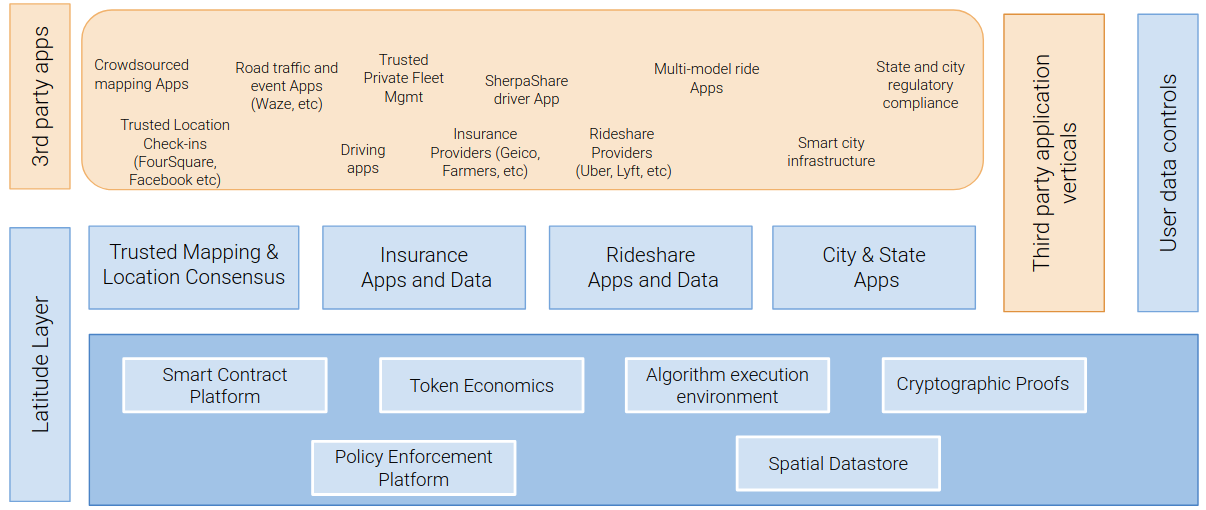
\includegraphics[width=0.90\textwidth]{latarch.png}
  \caption{Architecture of the Latitude Blockchain and associated platform ecosystem.}
    \label{fig:lat-arch}
\end{figure}

One of the central aspects of the Latitude blockchain is a geo-spatial datastore that fundamentally understands various
datatypes that are specific to transportation data. This datastore can use existing GIS databases that allow
de-centralized storage and access. The types of data include (i) georaphic data such as location (latitude, longitude),
(ii) mapping data such as roads, terrain, addresses, etc, (iii) sensor data such as driving data, driver score, miles
driven, route information, etc, (iv) multi-modal transport data such as biking, walking and other means of transport.
Each of these data types have very special characteristics which the underlying datastore can be optimized for and allow
for programming using what we call the {\em Latitude Smart Contract} framework. 

The datastore would include spatial, quad-tree or an R-tree based indexes for efficient querying and other operations that
most Geographic Information Systems (GIS) would support in a centralized manner today. It would also include functions
to compute heatmaps, driving maps and statistics such as Traffic predictions including real-time analytics. Depending on
how Latitude evolves, the datastore can include additional functionalities to support the data sharing among autonomous
vehicles since they use most of the similar datatypes mentioned above. The datastore would support circular, rectangular
and other range queries, K-nearest neighbor searches, route optimization algorithms, etc. Figure
\ref{fig:geo_spatial_query} shows some of the queries that such a datastore can support.

\begin{figure}[t]
    \centering
    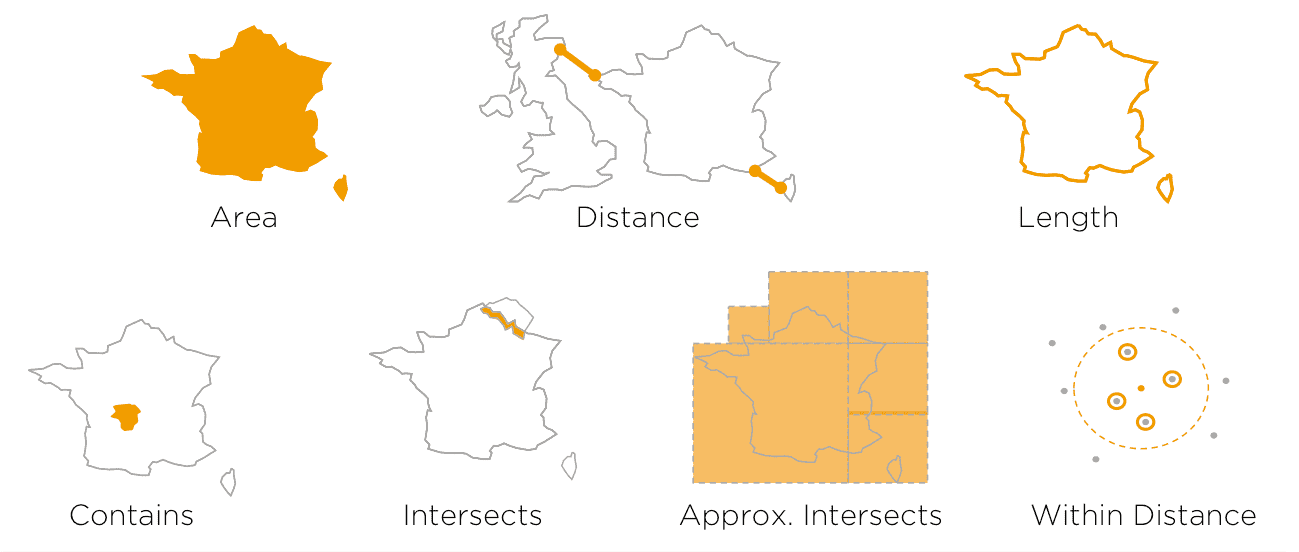
\includegraphics[width=0.90\textwidth]{geospatial_query.png}
  \caption{Examples of Geo-spatial queries that a spatial datastructure can support on the Latitude blockchain.}
    \label{fig:geo_spatial_query}
\end{figure}


Datastore
 - Optimized for Geographic, Geo-spatial data.
 - Location, Mapping data and computation.
 - Ability to Store, index, query and build smart contracts optimized for such data.
 - Support for various spatial indexes.
 - Location heatmaps.
 - Indexing road and driving data.
 - Primitives for storing driving data for autonomous vehicles

\noindent
{\textsf Strong crytographic foundation:}
Standard data encryption techniques allow for security guarantees in Latitude. Anonymity guarantees are provided using
privacy-preserving set operations such as given in \cite{kissner_set}, with suitable modifications to
anonymize spatial data which have user-location considerations \cite{divanis_kanon,xu_loc_anon}.
Cryptographic primitives for:
 - Security and privacy of data.
 - Anonymity guarantees using cryptographic set operations.
 - Enforcement of privacy when sharing data.
 - Sharing of “computation” instead of data when possible.
 - For eg: Sharing of DriverScore using a vetted algorithm.
 - Sharing proximity to a landmark instead of lat/lng.
 - Ability to find bad actors.
 - Detect privacy, anonymity and security violations.

\noindent
{\textsf Latitude Smart contract system:}

Smart contract system for Transportation applications.
 - Ability to convert “policies” such as GDPR into smart contract code.
 - Example, self destruct data after a time period.
 - Sandboxed trusted execution environment:
 - For algorithms:
   - DriverScore, Location heatmaps, Statistics.
   - Enforcing or verifying privacy and other govt policies/regulations.

Cryptographic proofs for applications:
 - Proof of Location. 
 - Proof of ride. 
 - Proof of mapping 
      (road/landmark exists or does not exist).
 - Proof of driver score 
 - Open, trusted, understood driver score computation algorithms.
 - Cryptographic proofs can be shared among entities, safely, securely.

\noindent
\subsection{Cryptoeconomics and Governance:}
Cryto-economics refers to the mechanics of the protocol underlying the blockchain operations which creates incentives
for the various stakeholders. For example, in the Latitude Blockchain it is possible to reward users for sharing their data
for certain purposes. For example, users can be rewarded if they share traffic data or accident information or better
routes. This is similar to the Waze model but creates legitimate rewards for users that have meaningful value outside
the Waze application. For an overview of cryptoeconomics in the blockchain space, please see \cite{sinclair_crypto}.

The core building block of the cryptoeconomics in Latitude is the Latitude Token, or LAT. This will be transacted in
each and every micro-transaction that takes place on the blockchain to create the right incentives, enforce smart
contracts and penalize Byzantine behavior. One of the fundamental design principles behind the protocol for the LAT
token is to create incentives assuming nodes are greedy and are interested in maximizing their gain. We will also build
safeguards against reasonable amount of collusion among nodes to subvert the system. The design is crafted such that the
best way for a node to maximize its revenue would be to participate with full honesty.

Latitude shall employ a Proof of Stake model (delegated or non-delegted) for particpation and core node-level mining. This mechanism has recently
gained popularity among a notable number of blockchains \cite{dpos_steemit}. This also allows for deposit slashing as a
technique to tackle Byzantine behavior. Latitude will employ techniques such as Minimal Slashing \cite{buterin_slashing}
for Byzantine fault tolerance and safety under distributed asynchronous operation.


Governance refers to a decentralized manner in which decisions are made using a consensus mechanism on the blockchain.
Decisions include basic constructs whether a node can join or leave the network. Or it can include key decisions on
whether an upgrade should be mandated on every node, a given participant such as a data provider should be penalized. It
could also include issues where humans get involved, such as when a user complains of a loss of privacy or a breach in
contract.

Recently blockchains have been moving towards governance using a small set of participants, such as trusted miners in
the case of Stellar and Ripple \cite{stellar_gateway}. The EOS blockchain uses a similar concept of a core set of block
producers who are elected based on a nomination and voting process \cite{eos_producers}. For discussion around
Governance in Ethereum, refer to \cite{buterin_gov}. Latitude uses a similar concept of a {\em council} of participants.
These are entities (nodes or organizations) that have demonstrated participating using earned trust through honest
operation, accumulating stake, demonstrated good intent and establishing trust. Some members of this council might
include the core Latitude developers which allows them to implement operations such as updates, bug fixes and so on. The
council members shall be elected using the an election protocol on the blockchain. It might be possible to directly
nominate certain council members such as regulatory bodies who have general interest in user rights, privacy and
enforcement. 

 - Crypto-incentives for honest operation.
 - Penalties for malicious intent.
 - Governance based on consensus and roles using a council.
 - Council members elected using voting, stake and established trust.
 - Some council members can have restricted access.
 - Eg: US govt can have voting rights on US data/users, etc.

User incentives:
 - Users have full control over their data and computation.
 - Users can issue or request proofs to carry over to other applications.
 - User’s have incentive to share data, participate in improving the common denominator.
 - Malicious intent, Byzantine behavior.
   - Can be detected using a combination of consensus and incentives.
   - Best interest of users to act honestly by design.


\noindent
{\textsf Performance considerations:}
Performance:
- Transaction speed. Data throughput. Storage capabilities.


%----------------------------------------------------------------------------- BIBLIOGRAPHY
%-----------------------------------------------------------------------------

\section{Author Bio}

\noindent {\bf Arunesh Mishra:} Dr. Mishra has 10 years of research and development experience in the Industry in
Location and Mapping. At Google, he built the Location platform used widely on Android and Chrome and Google Maps
applications. He was the core designer for the crowd-sourced algorithms that self-learn and power the location/mapping
for Google's mobile platform. The platform serves more than 2 Billion users daily. He holds a PhD, 30 issued patents and
22 pending patents today many of which are based on the physical layer mechanics of computing location and mapping. He
was won Best Paper awards at top ACM conferences and has over 30+ conference publications. He has widely contributed to
open source software used on standard Linux distributions today. He has also built the largest mobile peer-peer network
infrastructure for iOS/Android via Google Play Games offering.




\section{References}
\bibliography{latitude.bib}

\end{document}
